\documentclass{article}
\makeatletter
\renewcommand*\l@section{\@dottedtocline{2}{.5em}{2.3em}}
\renewcommand*\l@subsection{\@dottedtocline{2}{2.7em}{2.3em}}
\makeatother
\addtolength{\textwidth}{5cm}
\addtolength{\hoffset}{-2.5cm}
\addtolength{\voffset}{-1cm}
\addtolength{\textheight}{2.5cm}
%\usepackage{pdfsync}
\usepackage{fancyhdr}
\pagestyle{fancy}
% with this we ensure that the chapter and section
% headings are in lowercase.
% \renewcommand{\chaptermark}[1]{%
%         \markboth{#1}{}}
\renewcommand{\sectionmark}[1]{%
        \markright{\thesection\ #1}}
\fancyhf{} % delete current header and footer
\fancyhead[LO,RE]{\bfseries\thepage}
%\fancyhead[RO]{\bfseries\rightmark}
\fancyhead[LE,RO]{\bfseries\rightmark}
\renewcommand{\headrulewidth}{0.5pt}
\renewcommand{\footrulewidth}{0pt}
\addtolength{\headheight}{0.5pt} % space for the rule
\fancypagestyle{plain}{%
   \fancyhead{} % get rid of headers on plain pages
   \renewcommand{\headrulewidth}{0pt} % and the line
}
\usepackage{pstricks}
\usepackage{animate}
\usepackage{pstricks-add}
\usepackage{multido}
\usepackage{color}
\definecolor{myblue}{rgb}{0.02,0.04,0.48}
\definecolor{lightblue}{rgb}{0.61,.8,.8}
\definecolor{myred}{rgb}{0.65,0.04,0.07}
\definecolor{lightgray}{gray}{0.6}
\definecolor{mygreen}{rgb}{0,.43,0}
\usepackage{fancybox}
\usepackage{fancyvrb}
\usepackage{setspace}
\usepackage{perpage}
\usepackage{persianpoem}
\newenvironment{myverb}{\begin{Verbatim}[frame=single,numbers=left,framerule=1mm,rulecolor=\color{red},fillcolor=\color{yellow},framesep=3mm,showspaces=true,commandchars=+\[\]]}{\end{Verbatim}}
\usepackage{xepersian}
\settextfont[Scale=1.2]{XB Zar}
\setdigitfont[Scale=1.2]{XB Zar}
\setromantextfont[Scale=1.2]{Linux Libertine}
\defpersianfont\nastaliq[Scale=1.8]{IranNastaliq}
\defromanfont\linlib[Scale=1.5]{Linux Libertine}
%\addtolength{\hoffset}{-2cm}
%\addtolength{\textwidth}{3cm}
\newcommand{\textblue}[1]{{\addfontfeature{Color=0000FF}#1}}
\numberwithin{equation}{section}
\numberwithin{table}{section}
\onehalfspacing
\newcommand\femph[1]{«#1»}
\frenchspacing
\newcommand\LRcite[1]{\LR{\rmfamily{\cite{#1}}}}


\begin{document}

\thispagestyle{empty}

\noindent
\begin{LTR}
\begin{pspicture}(0,13.5)(\linewidth,0)
  \psline[linewidth=3mm,linecolor=mygreen](0,13.5)(\linewidth,13.5)
  \rput(\linewidth,13.5)
    {\pspolygon*(-3.6,0)(-1.4,0)(0,-1.4)(0,-3.6)}
  \rput(\linewidth,13.5)
    {\rput{-45}(-1,-1){\Large\textbf{\white \rl{نسخهٔ}}}}
  \rput(\linewidth,13.5)
    {\rput{-45}(-1.5,-1.5){\Large\textbf{\white \rl{۰/۱۶۳}}}}

  \rput[l](13,3.7){\textsl{\huge \rl{راهنمای بستهٔ}}}
  \psline[linewidth=3mm,linecolor=myred](0,3)(\linewidth,3)
  \psline[linewidth=3mm,linecolor=myred](0,0)(\linewidth,0)
  \rput[b](0.5\linewidth,5)
    {
\includegraphics[height=0.3\textheight]{iran.jpg}}
  \rput[l](0,1.5){\psscaleboxto(\textwidth,2){\rl{زی‌پرشین}}}

\end{pspicture}
\end{LTR}

\vfill\noindent
{{\huge \textbf{گروه فارسی‌--لاتک}} \hfill
{\large\textsl{وفا خلیقی، مهدی امیدعلی، و مصطفی واحدی}}}
\newpage
\pagenumbering{harfi}
\section*{مقدمه}
\newpage
\tableofcontents
\newpage
\listoftables
\newpage
\listoffigures
\newpage
\pagenumbering{persian}
\pagestyle{fancy}

\section{نمونهٔ فایل ورودی}
 یک نمونه فایل ورودی می‌تواند به صورت زیر باشد.


\begin{Verbatim}[frame=single,numbers=left,framerule=1mm,rulecolor=\color{red},fillcolor=\color{yellow},framesep=3mm,showspaces=true,commandchars=+\(\)]
+color(myblue)\documentclass{book}
+color(lightblue)\usepackage{xepersian}
+color(myred)\settextfont[Scale=1]{XB Zar}
+color(myred)\setromantextfont[Scale=1]{Junicode}
+color(myred)\setdigitfont[Scale=1]{XB Zar}
+color(mygreen)\title{+rl(عنوان نوشتار)}
+color(mygreen)\author{+rl(نام نویسنده)}
+color(lightgray)\begin{document}
\maketitle
\tableofcontents
\chapter{+rl(فصل اول)}
\section{+rl(بخش اول)}
...
+color(lightgray)\end{document}
\end{Verbatim}

همانطور که می‌بینید شکل فایل ورودی هیچ‌گونه تفاوتی با یک فایل استاندارد لاتک ندارد. تنها ممکن است فرمانهای خط سوم، چهارم، و پنجم این فایل نمونه برای شما 
نا آشنا باشند که در قسمتهای بعد به توضیح آنها می‌پردازیم. به طور کلی در استفاده از طبقه‌های استاندارد لاتک به جز فراخوانی بستهٔ \lr{\XePersian} هیچ 
کار اضافه‌ای لازم نیست که انجام دهید. تنها به عنوان یک توصیه، سعی کنید 

\centerline{\shadowbox{\nastaliq\textblue{
 این بسته آخرین بسته‌ای باشد که فراخوانی می‌کنید و فرمان‌های خود را بعد از فراخوانی این بسته قرار دهید.}} }

همچنین توجه داشته باشید که 
بسته‌های زیر به طور خودکار فراخوانی می‌شوند و شما نباید آنها را مستقیماً در فایل فراخوانی کنید.

\centerline{\shadowbox{\lr{amsmath, amssymb, amsthm, graphicx.}}}

همچنین بسته \lr{\XePersian} هنوز قابلیت استفاده از طبقهٔ \lr{memoir} را ندارد، ولی در آینده این امکان نیز افزوده خواهد شد. 
\section{فرمانهای بسته}
در این قسمت تعدادی از فرمانهای مفید را که لازم است بدانید شرح می‌دهیم.  در جدول \ref{commands} فرمانهای بسته را مشاهده
می‌کنید. همچنین در بسته چند نوع شمارنده تعریف شده است که در جدول \ref{counters} مشاهده می‌کنید.



\begin{table}[!hbp]
\begin{center}
\begin{tabular}{|r|l|}
\hline
 فرمان & شرح\\
 \hline
 \verb+\settextfont[...]{...}+&قلم فارسی متن را مشخص می‌کند.\\
 \hline
 \verb+\setromantextfont[...]{...}+&قلم انگلیسی متن را مشخص می‌کند.\\
 \hline
 \verb+\setdigitfont[...]{...}+&قلم ارقام را در فرمول‌ها مشخص می‌کند.\\
 \hline
 \verb+\defpersianfont\fontname[...]{...}+&یک قلم فارسی را مشخص می‌کند.\\
\hline
 \verb+\defromanfont\fontname[...]{...}+&یک قلم انگلیسی را مشخص می‌کند.\\
\hline
\verb+\footnote{...}+&برای درج یک پانوشت فارسی \\
\hline
\verb+\Footnote{...}+&برای درج یک پانوشت انگلیسی \\
\hline
\verb+\today+&درج تاریخ جاری خورشیدی\\
\hline
\verb+\englishtoday+&درج تاریخ جاری میلادی\\
\hline
\verb+\rldblcolumn+&ترتیب ستونها را در یک متن چندستونی از راست‌ به ‌چپ می‌کند (پیش‌فرض)\\
\hline 
\verb+\lrdblcolumn+&ترتیب ستونها را در یک متن چند‌ستونی از چپ ‌به ‌راست می‌کند \\
\hline
\verb+\twocolumnstableofcontents+ & فهرست مطالب را در دو ستون می‌چیند (نیاز به فراخوانی \verb+fmultico+ دارد)\\
\hline
\verb+\lr{...}+&یک متن کوتاه انگلیسی را در یک پاراگراف فارسی قرار می‌دهد\\
\hline
 \verb+\rl{...}+&یک متن کوتاه فارسی را در یک پاراگراف انگلیسی قرار می‌دهد\\
\hline
\verb+\begin{LTR}+&شروع محیط چپ‌به‌راست\\
 \verb+\end{LTR}+&پایان محیط  چپ‌به‌راست\\
\hline
\verb+\begin{RTL}+&شروع محیط راست‌به‌چپ\\
\verb+\end{RTL}+&پایان محیط راست‌به‌چپ\\
\hline
\verb+\begin{roman}+&شروع محیط انگلیسی مجهز به قلم انگلیسی متن\\
 \verb+\end{roman}+&پایان محیط انگلیسی\\
\hline
\verb+\begin{persian}+&شروع محیط فارسی مجهز به قلم فارسی متن\\
\verb+\end{persian}+&پایان محیط فارسی\\
\hline
\verb+\Roman+&برای درج کتاب‌نامه‌های انگلیسی\\
\hline
\verb+\Persian+&برای درج کتاب‌نامه‌های فارسی\\
\hline
 \verb+\rmfamily+&قلم انگلیسی را برای حروف‌چینی استفاده می‌کند (پیش‌فرض محیط \verb+roman+)\\
\hline
\verb+\farsifont+&قلم فارسی را برای حروف‌چینی استفاده می‌کند (پیش‌فرض محیط \verb+persian+) \\
\hline
 \verb+\PersianFootNum+&شمارهٔ پانوشت‌های انگلیسی را به صورت فارسی درج می‌کند (پیش‌فرض )\\
\hline
 \verb+\RomanFootNum+&شمارهٔ پانوشت‌های انگلیسی را به صورت انگلیسی درج می‌کند.\\
\hline
 \verb+\RomanBibNum+&شمارهٔ مراجع انگلیسی را به صورت انگلیسی درج می‌کند (پیش‌فرض)\\
\hline
 \verb+\PersianBibNum+&شمارهٔ مراجع انگلیسی را به صورت فارسی درج می‌کند.\\
\hline
\end{tabular}
\end{center}
\caption{فرمان‌ها}\label{commands}
\end{table}

\begin{table}[!hbp]
\begin{center}
\begin{tabular}{|r|l|}
\hline
 شمارنده & شرح\\
\hline
\verb+arabic+&شمارندهٔ عربی اصلی لاتک برای سازگاری با بسته از نو تعریف شده است. \\
\hline
 \verb+persian+&همان اثر شمارنده \verb+arabic+ اصلی لاتک را دارد.\\
\hline
\verb+adadi+& شمارنده را به صورت یک، دو، سه، \ldots تغییر می‌دهد. \\
\hline
\verb+harfi+&شمارنده را به صورت الف\char"200D، ب، پ، \ldots تغییر می‌دهد.\\
\hline
\verb+tartibi+&شمارنده را به صورت اول، دوم، سوم، و \ldots تغییر می‌دهد.\\
\hline
\end{tabular}
\end{center}
\caption{شمارنده‌ها}\label{counters}
\end{table}

\section{استفاده از قلمهای مختلف}
بستهٔ \lr{fontspec}، که به صورت خودکار فراخوانی می‌شود، امکان استفاده از قلمهای موجود در سیستم را فراهم می‌کند. برای استفاده از \lr{\XePersian}
لازم است که حداقل یک قلم اصلی حروف‌چینی متن را مشخص کنید. این کار را با فرمان زیر انجام می‌دهیم:
\begin{Verbatim}[frame=single,numbers=left,framerule=1mm,rulecolor=\color{red},fillcolor=\color{yellow},framesep=3mm,showspaces=true,commandchars=+()]
\settextfont[Scale=+rl(مقیاس)]{+rl(نام قلم)}
\end{Verbatim}
به عنوان مثال با فرمان 
\begin{Verbatim}[frame=single,numbers=left,framerule=1mm,rulecolor=\color{blue},framesep=3mm,showspaces=true,commandchars=+()]
\settextfont[Scale=1]{XB Zar}
\end{Verbatim}

قلم \lr{XB Zar} را با مقیاس بزرگی \lr{1} به عنوان قلم اصلی فارسی معرفی می‌کند. گزینهٔ \verb+Scale=1+ اختیاری است و مشخص می‌کند که قلم با چه سایزی مورد استفاده قرار گیرد. توجه داشته باشید که \lr{XB Zar} عنوان قلمی است که باید روی سیستم شما نصب باشد. اگر سیستم شما ویندوز است قلم مورد استفاده باید در پوشهٔ
\fbox{\lr{C:$\backslash$windows$\backslash$fonts}}
موجود باشد. این قلم یکی از قلمهای سری ایکس ساخته شده توسط گروه کاربران فارسی اپل-مکینتاش است که بسیار کامل هستند و توصیه می‌شود از این قلم‌ها استفاده شود. برای دریافت آنها به آدرس زیر مراجعه کنید:

\centerline{\fbox{\texttt{http://wiki.irmug.org/index.php/X\_Series\_2}}}
برای اینکه قلم نگارش ارقام در فرمول‌ها را مشخص کنید از فرمان زیر استفاده کنید:
\begin{Verbatim}[frame=single,numbers=left,framerule=1mm,rulecolor=\color{red},fillcolor=\color{yellow},framesep=3mm,showspaces=true,commandchars=+()]
\setdigitfont[Scale=+rl(مقیاس)]{+rl(نام قلم)}
\end{Verbatim} 
و قلم نگارش متن‌های انگلیسی را با فرمان زیر مشخص می‌کنیم:
\begin{Verbatim}[frame=single,numbers=left,framerule=1mm,rulecolor=\color{red},fillcolor=\color{yellow},framesep=3mm,showspaces=true,commandchars=+()]
\setromantextfont[Scale=+rl(مقیاس)]{+rl(نام قلم)}
\end{Verbatim}

همچنین می‌توانید هر تعداد قلم فارسی دلخواه را معرفی کنید و در نوشتار خود مورد استفاده قرار دهید. فرمان انجام این کارها به صورت زیر است:
\begin{Verbatim}[frame=single,numbers=left,framerule=1mm,rulecolor=\color{red},fillcolor=\color{yellow},framesep=3mm,showspaces=true,commandchars=+()]
\defpersianfont\fontname[Scale=+rl(مقیاس)]{+rl(نام قلم)}
\defromanfont\fontname[Scale=+rl(مقیاس)]{+rl(نام قلم)}
\end{Verbatim}
به عنوان مثال فرمان 


\begin{Verbatim}[frame=single,numbers=left,framerule=1mm,rulecolor=\color{blue},framesep=3mm,showspaces=true,commandchars=+()]
\defpersianfont\nastaliq[Scale=2]{IranNastaliq}
\end{Verbatim}
قلم نستعلیق را برای نوشتار معرفی می‌کند و در متن می‌توانید به دو صورت از آن استفاده کنید: 
\begin{itemize}
\item 
در یک محیط \lr{RTL} به صورت زیر

\begin{Verbatim}[frame=single,numbers=left,framerule=1mm,rulecolor=\color{blue},framesep=3mm,showspaces=true,commandchars=+\[\]]
\begin{RTL}
\nastaliq
+rl[نمونه متن با قلم نستعلیق]
\end{RTL}
\end{Verbatim}


که اثر آن همانند متن زیر است:

\begin{center}\fbox{\Large\nastaliq نمونه متن با قلم نستعلیق}\end{center}
این روش مناسب نوشتن یک پاراگراف یا بیشتر است.
\item
یا به صورت ساده به شکل زیر از قلم تعریف شده استفاده کنید

\begin{Verbatim}[frame=single,numbers=left,framerule=1mm,rulecolor=\color{blue},framesep=3mm,showspaces=true,commandchars=+\[\]]
\nastaliq{+rl[نمونه متن با قلم نستعلیق]}
\end{Verbatim}
که اثر این فرمان هم مشابه قبل است. این روش مناسب نوشتن یک متن کوتاه با قلم تعریف شده است.

\end{itemize}
به روش مشابه می‌توانید هر تعداد قلم انگلیسی دلخواه تعریف کنید و از آنها استفاده کنید. فرمان
\begin{Verbatim}[frame=single,numbers=left,framerule=1mm,rulecolor=\color{red},fillcolor=\color{yellow},framesep=3mm,showspaces=true,commandchars=+()]
\defromanfont\fontname[Scale=+rl(مقیاس)]{+rl(نام قلم)}
\end{Verbatim}

وظیفهٔ تعریف قلم‌های مختلف انگلیسی را به عهده دارد. به عنوان مثال با فرمان 
\begin{Verbatim}[frame=single,numbers=left,framerule=1mm,rulecolor=\color{blue},framesep=3mm,showspaces=true,commandchars=+()]
\defromanfont\linlib[Scale=1.5]{Linux Libertine}
\end{Verbatim}
قلم 
\lr{Linux Libertine} با مقیاس بزرگی \lr{1.5} معرفی می‌شود که می‌توان از آن به صورت زیر استفاده کرد:

\begin{Verbatim}[frame=single,numbers=left,framerule=1mm,rulecolor=\color{blue},framesep=3mm,showspaces=true,commandchars=+\[\]]
\begin{LTR}
\linlib
Sample text with Linux Libertine font
\end{LTR}
\end{Verbatim}

که اثر آن به شکل زیر است:


\begin{LTR}\centerline{\fbox{\linlib
Sample text with Linux Libertine font
}}\end{LTR}

\section{گزینه‌های بستهٔ \lr{\XePersian}}
به دلیل تنوع روش‌های حروف‌چینی پایان‌نامه‌ها و کتاب‌های فارسی، بستهٔ \lr{\XePersian} دارای امکاناتی است که با استفاده از آنها می‌توانید نوشتار خود را به سبک دلخواه طراحی کنید. 
\subsection{پانوشت‌ها}
از فرمان‌های 
\verb+\footnote+ 
و 
\verb+\Footnote+ 
برای نوشتن پانوشت‌های فارسی و انگلیسی (به ترتیب) استفاده می‌شود. سبک پیش‌فرض بسته این است که شمارهٔ تمام پانوشت‌ها به صورت فارسی نوشته می‌شود و بسته به اولین پانوشت هر صفحه، خط حائل در سمت مناسب قرار داده می‌شود.  اگر می‌خواهید شمارهٔ پانوشت‌های انگلیسی در کل نوشتار به صورت عدد انگلیسی باشد از گزینهٔ 
\verb+RomanFootNum+ 
در هنگام فراخوانی بسته به صورت زیر استفاده کنید
\begin{Verbatim}[frame=single,numbers=left,framerule=1mm,rulecolor=\color{blue},framesep=3mm,showspaces=true,commandchars=+()]
\usepcackage[RomanFootNum]{xepersian}
\end{Verbatim}
همچنین در خود نوشتار هر جا که خواستید شمارهٔ پانوشت‌ها فارسی یا انگلیسی باشد از فرمان‌های 
\verb+\PersianFootNum+ 
یا 
\verb+\RomanFootNum+ 
(به ترتیب) استفاده کنید.
به عنوان مثال
این یک پانوشت فارسی است \footnote{شمارهٔ پانوشت فارسی است.} و این هم یک پانوشت انگلیسی است% 
\Footnote{The number of the footnote is persian.} 
که شمارهٔ آن فارسی است. حال فرمان 
\verb+\RomanFootNum+
را در مستند قرار می‌دهیم.
\RomanFootNum
این یک پانوشت انگلیسی است%
\Footnote{The number of the footnote is roman.} 
که شمارهٔ آن انگلیسی است. برای برگشت به حالت اولیه فرمان 
\verb+\PersianFootNum+
را در مستند قرار می‌دهیم.
\PersianFootNum
و حال این یک پانوشت دیگر انگلیسی است%
\Footnote{The number of the footnote is persian again.}
که شمارهٔ آن فارسی شده است.
\subsection{کتاب‌نامه}
دو محیط \verb+\Persian+ و \verb+\Roman+ برای درج مراجع فارسی و انگلیسی تعریف شده است. بنابراین برای نوشتن کتاب‌نامهٔ خود به صورت زیر می‌توانید عمل کنید

\begin{Verbatim}[frame=single,numbers=left,framerule=1mm,rulecolor=\color{blue},framesep=3mm,showspaces=true,commandchars=+()]
\begin{thebibliography}
\Persian
\bibitem{hafez}+rl(دیوان حافظ، انتشارات سروش).
\Roman
\bibitem{faust}  Johann Wolfgang von Goethe, Faust.
\end{thebibliography}
\end{Verbatim}
در این صورت کتاب‌نامهٔ شما به صورت زیر حروف‌چینی می‌شود:

\bigskip

\centerline{\fbox{
\begin{minipage}[r]{10cm}
\begin{thebibliography}
\Persian
\bibitem{hafez} دیوان حافظ، انتشارات سروش.
\Roman
\bibitem{faust} Johann Wolfgang von Goethe, Faust.
\end{thebibliography}
\end{minipage}
}}
\bigskip

اگر بخواهید شمارهٔ مراجع انگلیسی به صورت عدد فارسی باشد از فرمان \verb+\PersianBibNum+ در مستند خود استفاده کنید در این صورت کتاب‌نامهٔ شما به صورت زیر چیده می‌شود:
\bigskip

\PersianBibNum
\centerline{\fbox{
\begin{minipage}[r]{10cm}
\begin{thebibliography}
\Persian
\bibitem{hafez} دیوان حافظ، انتشارات سروش.
\Roman
\bibitem{faust} Johann Wolfgang von Goethe, Faust.
\end{thebibliography}
\end{minipage}
}}
\bigskip
\RomanBibNum

به همین ترتیب می‌توانید از فرمان \verb+\RomanBibNum+ استفاده کنید و شمارهٔ مراجع انگلیسی را به صورت عدد انگلیسی درج کنید. این دو فرمان را در هر جای مستند که وارد کنید اثر خود را از آن نقطه به بعد ظاهر می‌کنند ولی اگر می‌خواهید یکی از این دو سبک را در نوشتار خود داشته باشید (که اغلب این‌گونه است) بهتر است از گزینه‌های 
\verb+RomanBibNum+ و یا \verb+PersianBibNum+
هنگام فراخوانی بستهٔ \lr{\XePersian} استفاده کنید. گزینهٔ 
\verb+RomanBibNum+
گزینهٔ پیش‌فرض است و بنابراین اگر می‌خواهید کتاب‌نامهٔ شما به فرم دوم چاپ شود از فرمان زیر در سرآغاز فایل خود استفاده کنید:

\begin{Verbatim}[frame=single,numbers=left,framerule=1mm,rulecolor=\color{blue},framesep=3mm,showspaces=true,commandchars=+()]
\usepackage[PersianBibNum]{xepersian}
\end{Verbatim}

\subsection*{خلاصه}
اگر بخواهید مثلاً شمارهٔ پانوشت‌های انگلیسی به صورت انگلیسی باشد و شمارهٔ مراجع انگلیسی به صورت فارسی باشد از فرمان زیر استفاده کنید

\begin{Verbatim}[frame=single,numbers=left,framerule=1mm,rulecolor=\color{blue},framesep=3mm,showspaces=true,commandchars=+()]
\usepackage[PersianBibNum,RomanFootNum]{xepersian}
\end{Verbatim}
\section{حروف‌چینی شعر}
برای حروف‌چینی شعر باید فرمان زیر را در سرآغاز فایل خود قرار دهید:

\begin{Verbatim}[frame=single,numbers=left,framerule=1mm,rulecolor=\color{blue},framesep=3mm,showspaces=true,commandchars=+()]
\usepackage{persianpoem}
\end{Verbatim}
بعد از این کار به راحتی می‌توانید شعر را حروف‌چینی کنید.

{\nastaliq\doublespacing
\begin{oldpoem}

هله رفتیم و گرانی ز جمالت بردیم&
جهت توشهٔ ره ذکر وصالت بردیم\\
تا که ما را و ترا تذکرهٔ خوش باشد&
دل خسته بتو دادیم و خیالت بردیم\\
آن خیال رُخ خوبت که قمر بندهٔ اوست&
وان خَم ابروی مانند هلالت بردیم\\
و آن شکرخندهٔ خوبت که شکر تشنهٔ اوست&
ز شکر خانهٔ مجموع خصالت بردیم\\
چون کبوتر چو بپریم بتو بازآییم&
زانکه ما این پَر و بال از پَر و بالت بردیم\\
هر کجا پرد فرعی، بسوی اصل آید&
هر چه داریم هم از عزّ و جلالت بردیم\\
شمس تبریز شنو خدمت ما را زصبا&
گر شمالست و صبا هم ز شمالت بردیم

\end{oldpoem}
}
شعر بالا با کد زیر تولید شده است:

\begin{Verbatim}[frame=single,numbers=left,framerule=1mm,rulecolor=\color{blue},framesep=3mm,showspaces=true,commandchars=+()]
\begin{oldpoem}
+rl(هله رفتیم و گرانی ز جمالت بردیم)&
+rl(جهت توشهٔ ره ذکر وصالت بردیم)\\
+rl(تا که ما را و ترا تذکرهٔ خوش باشد)&
+rl(دل خسته بتو دادیم و خیالت بردیم)\\
+rl(آن خیال رُخ خوبت که قمر بندهٔ اوست)&
+rl(وان خَم ابروی مانند هلالت بردیم)\\
+rl(و آن شکرخندهٔ خوبت که شکر تشنهٔ اوست)&
+rl(ز شکر خانهٔ مجموع خصالت بردیم)\\
+rl(چون کبوتر چو بپریم بتو بازآییم)&
+rl(زانکه ما این پَر و بال از پَر و بالت بردیم)\\
+rl(هر کجا پرد فرعی، بسوی اصل آید)&
+rl(هر چه داریم هم از عزّ و جلالت بردیم)\\
+rl(شمس تبریز شنو خدمت ما را زصبا)&
+rl(گر شمالست و صبا هم ز شمالت بردیم)\\
\end{oldpoem}
\end{Verbatim}


این محیط دارای حالت ستاره‌دار (\verb+oldpoem*+) نیز می‌باشد که اثر آن به صورت زیر است.
\begin{oldpoem*}
هله رفتیم و گرانی ز جمالت بردیم&
جهت توشهٔ ره ذکر وصالت بردیم\\
تا که ما را و ترا تذکرهٔ خوش باشد&
دل خسته بتو دادیم و خیالت بردیم\\
آن خیال رُخ خوبت که قمر بندهٔ اوست&
وان خَم ابروی مانند هلالت بردیم\\
و آن شکرخندهٔ خوبت که شکر تشنهٔ اوست&
ز شکر خانهٔ مجموع خصالت بردیم\\
چون کبوتر چو بپریم بتو بازآییم&
زانکه ما این پَر و بال از پَر و بالت بردیم\\
هر کجا پرد فرعی، بسوی اصل آید&
هر چه داریم هم از عزّ و جلالت بردیم\\
شمس تبریز شنو خدمت ما را زصبا&
گر شمالست و صبا هم ز شمالت بردیم
\end{oldpoem*}
شعر بالا با کد زیر تولید شده است:

\section{حروف‌چینی چند‌ستونی}
برای حروف‌چینی یک متن در چند ستون از محیط زیر استفاده کنید. حداکثر تعداد ستونها ۵ است.

\begin{Verbatim}[frame=single,numbers=left,framerule=1mm,rulecolor=\color{blue},framesep=3mm,showspaces=true,commandchars=+()]
\begin{multicols}{+rl(تعداد ستون‌ها)}
.....
\end{multicols}
\end{Verbatim}

\section{محیط مورد فارسی}
محیط مورد برای استفاده در فارسی نیز تعریف شده است که در زیر مثال آنرا می‌بنید:

$$
\rcases{\mbox{مرد}\cr\mbox{زن}}\mbox{آدم}
$$

طرح بالا با کد زیر نوشته شده است.
\begin{Verbatim}[frame=single,numbers=left,framerule=1mm,rulecolor=\color{blue},framesep=3mm,showspaces=true,commandchars=+()]
$$\rcases{\mbox{+rl(مرد)}\cr\mbox{+rl(زن)}}\mbox{+rl(آدم)}$$
\end{Verbatim}


\section{تولید نمایه}
به همراه این بسته، فایلی ارائه شده است که شما را قادر می‌سازد به راحتی نمایه برای مستندتان فراهم کنید. خود بسته هیچ‌گونه محدودیتی با نمایه‌سازی ندارد،
ولی نرم‌افزار 
\lr{makeindex} هنگام مرتب کردن فایل نمایه، ترتیب بعضی از حروف را به درستی رعایت نمی‌کند. 
برای رفع این مشکل، استفاده از \lr{xindy} بجای \lr{makeindex} توصیه می‌شود.

اگر از تکلایو ۲۰۰۸ استفاده می‌کنید \lr{xindy} به طور خودکار روی سیستم شما نصب است. کافی است فایل \lr{persian.xdy} را که همراه این بسته 
ارائه شده است در دایرکتوری جاری قرار دهید و فرمانهای زیر را در خط فرمان اجرا کنید:

\begin{Verbatim}[frame=single,numbers=left,framerule=1mm,rulecolor=\color{blue},framesep=3mm,showspaces=true,commandchars=+()]
tex2xindy < filename.idx > filename.raw
xindy -I xindy -M persian.xdy filename.raw
\end{Verbatim}

\noindent بعد از انجام این کار، نمایهٔ مرتب شدهٔ شما آمادهٔ تزریق به مستند می‌شود.

توجه داشته باشید که اگر می‌خواهید از نمایه استفاده کنید، باید شمارندهٔ صفحه را در حالت \lr{\texttt{persian}} قرار دهید. البته شمارندهٔ صفحه به صورت 
پیش‌فرض در این حالت قرار دارد.
\section{فرمولهای ریاضی}
بسته با حروف‌چینی فرمولهای ریاضی هیچ‌گونه مشکلی ندارد و از آنجا که بسته‌های \lr{amsmath,amsthm,} و \lr{amssymb}  به طور خودکار فراخوانی می‌شوند،
اکیداً توصیه می‌شود از فرمانهای کلاف \lr{AMSLatex} استفاده کنید. توجه داشته باشید که محیط \texttt{eqnarray} کلا با بستهٔ \lr{amsmath}
مشکل دارد و به خصوص شمارهٔ فرمول نوشته شده با این محیط ناپایدار است. به جای این محیط، از محیط \texttt{align} استفاده کنید که 
حروف‌چینی آن از \texttt{eqnarray} بهتر است و شمارهٔ آن نیز بدون مشکل قابل ارجاع است.
\begin{align}
a^2+b^2&=\sin x\label{eq1}\\
2.1a+b&=\cos y\label{eq2}
\end{align}

فرمولهای بالا با کد زیر تولید شده‌اند.

\begin{roman}
\begin{verbatim}
\begin{align}
a^2+b^2&=\sin x\label{eq1}\\
1a+b&=\cos y\label{eq2}
\end{align}
\end{verbatim}
\end{roman}
ارجاع به فرمول \eqref{eq1} به صورت طبیعی امکان‌پذیر است. برای اطلاعات بیشتر به \femph{مقدمه‌ای نه‌چندان کوتاه بر \lr{\LaTeXe}}
%\footnote{قابل دسترسی از\texttt{http://www.ctan.org}} 
مراجعه کنید.
\section{تهیهٔ اسلاید با \lr{beamer}}
امکانات استفاده از طبقهٔ \lr{beamer} در حد مطلوبی برقرار است. برای استفادهٔ بهینه چند محیط جدید تعریف شده‌اند. 
\begin{Verbatim}[frame=single,numbers=left,framerule=1mm,rulecolor=\color{red},fillcolor=\color{yellow},framesep=3mm,showspaces=true,commandchars=+()]
\begin{+rl(بلوک)}{+rl(عنوان)}
...
\end{+rl(بلوک)}
\end{Verbatim}
با این فرمان یک بلوک عادی تشکیل می‌شود که جهت آن از راست به چپ است. به جای ''بلوک`` می‌توانید از ''بلوک‌مثال`` یا ''بلوک‌هشدار`` استفاده کنید.

\section{استفاده از \lr{PSTricks}}
تمامی امکانات استفاده از \lr{PSTricks} در بسته موجود است.
% \begin{LTR}
%   %-------------------- write timeline file ---------------------%
%   \newwrite\TimeLineFile
%   \immediate\openout\TimeLineFile=sinus.txt
%   \immediate\write\TimeLineFile{::0x0,1}%
%   %remaining frames: overlay filled circle at its current postion
%   \multido{\i=2+1}{90}{%
%     \immediate\write\TimeLineFile{%
%       ::\i % put filled circle on top
%   }}
%   \immediate\closeout\TimeLineFile
%   %------------------- assemble animation -----------------------%
%   \psset{xunit=\pstRadUnit,dashadjust=false}
%   \begin{animateinline}[controls,timeline=sinus.txt,
%     begin={\begin{pspicture}(-0.5,-1.5)(6.6,2)},
%     end={\end{pspicture}}]{24}
%     %---- static material: axes, labels, curve ----%
%     \psaxes[trigLabels,trigLabelBase=3]{->}(0,0)(-2mm,-1.5)(6.5,1.5)[t,-90][$y=\sin(t)$,0]
%     \psplot[xunit=1cm,linestyle=dashed,algebraic]{0}{\psPiTwo}{sin(x)}
%     \newframe
%     \multiframe{91}{n=0+4}{\psset{xunit=1cm,linecolor=blue}
%       \pscustom[xunit=1cm,fillcolor=blue!30,fillstyle=solid,
%         linestyle=none,algebraic,dimen=inner]{%
%         \psplot{0}{\n\space DegtoRad}{sin(x)}
%         \psline(!\n\space DegtoRad 0)
%       }
%       \psplot[xunit=1cm,linestyle=dashed,linecolor=black,
%          algebraic]{0}{\n\space DegtoRad}{sin(x)}
%       \psdot[opacity=0.4,dotsize=3mm](!\n\space dup DegtoRad exch sin)
%       \psline[linestyle=dashed](!\n\space dup DegtoRad exch sin)(!\n\space DegtoRad 0)
%     }
%   \end{animateinline}
% \end{LTR}




\appendix
\section{نصب ویرایشگر روی ویندوز}
برای استفاده از  \lr{\XePersian} باید  \lr{XeTeX} روی سیستم شما نصب باشد. اگر از \lr{MikTex 2.7} یا بالاتر، و یا از \lr{TeXLive 2008} 
و یا بالاتر استفاده می‌کنید، \lr{XeTeX} به طور خودکار روی سیستم شما نصب شده است. تنها کاری که باید در این صورت انجام دهید نصب و 
تنظیم یک ویرایشگر مناسب برای کار است. لیست کنترل زیر ابزارهای لازم را برای کار با این بسته به شما نشان می‌دهد.
\begin{enumerate}
\item توزیع مناسبی از \lr{\TeX} مانند \lr{Texlive}(\lr{2008} یا بالاتر) یا \lr{Miktex} (\lr{2.7} یا بالاتر).
\item نرم‌افزار مناسب ویرایش متنهای یونیکد (در ویندوز \lr{notepad++}\footnote{قابل دریافت از \LR{\texttt{http://notepad-plus.sourceforge.net/}}} و در لینوکس \lr{gedit}).
\item نرم‌افزار مناسب نمایش فایلهای پی.دی.اف (در ویندوز توصیه می‌شود از \lr{SumatraPDF}\footnote{قابل دریافت از \lr{\texttt{http://www.parsilatex.org/pdfreader/SumatraPDF.rar}}} به جای آکروبات ریدر استفاده شود).
\end{enumerate}
از آنجا که کاربران ایرانی معمولا از ویندوز استفاده می‌کنند و با توجه به اینکه یک ویرایشگر مناسب زندگی را برای کاربر بسیار راحت می‌کند، در ادامه 
روش نصب و تنظیم ویرایشگر مناسب را در ویندوز به طور کامل شرح می‌دهیم. توجه داشته باشید که فرض بر این است یک توزیع مناسب از تک و 
همچنین \lr{SumatraPDF} روی سیستم شما نصب است. 

فایل نصب‌کنندهٔ \lr{notepad++} را اجرا کنید ( توجه داشته باشید که جدیدترین نسخه این فایل را از صفحهٔ خانگی این نرم‌افزار دریافت کرده باشید). 
افزونهٔ (\lr{plugin}) \verb+NppExec.dll+ را نیز از صفحهٔ خانگی \lr{notepad++} دریافت کنید و آن را در پوشهٔ 
\begin{roman}\verb|C:\Program Files\Notepad++\plugins|\end{roman}
قرار دهید.
سپس به صورتی که در شکلهای زیر نشان داده شده است نرم‌افزار را نصب و تنظیم کنید.

\centerline{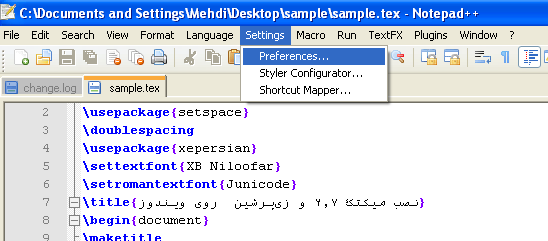
\includegraphics[height=5cm]{notepad1.PNG}}
\centerline{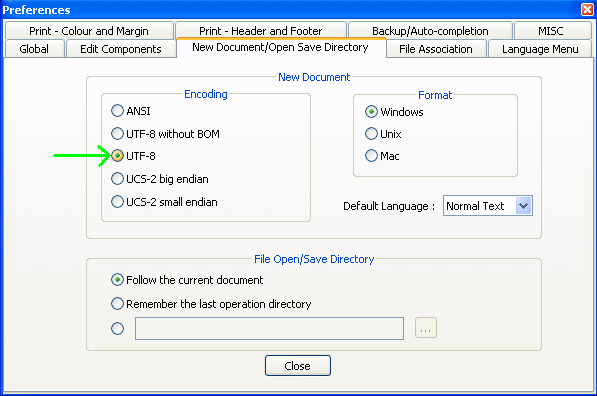
\includegraphics[height=7cm]{notepad2.PNG}}
\centerline{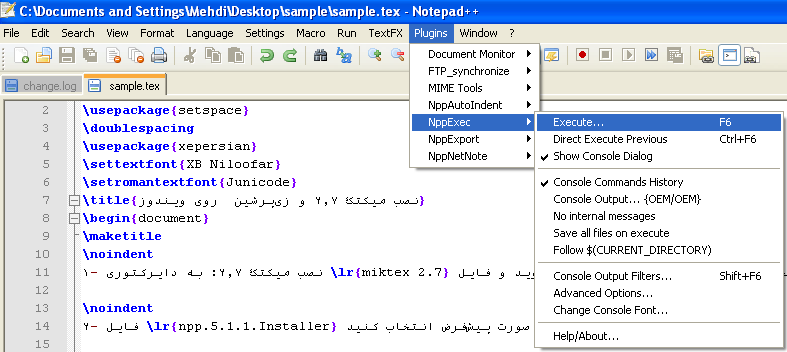
\includegraphics[height=6cm]{notepad3.PNG}}
\centerline{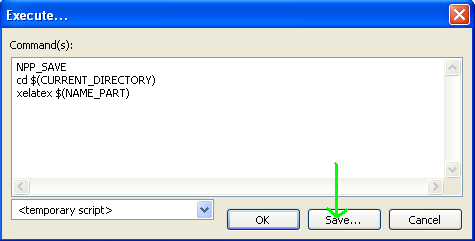
\includegraphics[height=5cm]{notepad4.PNG}}
\centerline{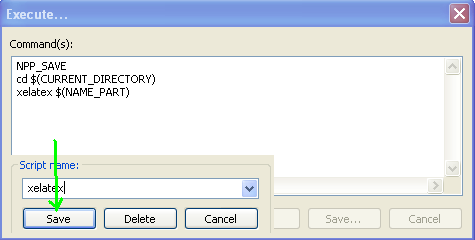
\includegraphics[height=6cm]{notepad5.PNG}}
\centerline{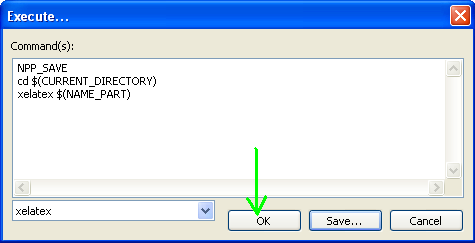
\includegraphics[height=5cm]{notepad6.PNG}}

متنی که در آخرین مرحله باید وارد کنید و حاصل را با عنوان \lr{xelatex} ذخیره کنید متن زیر است که می‌توانید به راحتی آن را از همین فایل پی.دی.اف 
کپی کنید و در پنجره‌ای که ظاهر شده است بچسبانید(به کوچک و بزرگ بودن حروف و همچنین فاصله بین کلمات دقت کنید):

\setLR
\small{
\begin{verbatim}
NPP_SAVE
cd $(CURRENT_DIRECTORY)
xelatex $(NAME_PART)
\end{verbatim}
}
\setRL
برای استفادهٔ بهینه از این ویرایشگر، بهتر است راهنمای آنرا مطالعه کنید. فقط به عنوان یک مطلب که ممکن است برای شما مفید باشد، هنگام ویرایش متنهای فارسی،
با فشردن \lr{ALT+CTRL+R} صفحه نمایش از راست به چپ قرار می‌گیرد و بنابراین کار شما راحت‌تر می‌شود. برای برگشتن به حالت چپ‌به‌راست کافی است
\lr{ALT+CTRL+L} را فشار دهید. بعد از انجام این کارها به راحتی می‌توانید با فشردن کلید \verb+F6+ فایل ورودی خود را پردازش کنید.

برای اینکه بتوانید از داخل ویرایشگر فایل پی.دی.اف خروجی را مشاهده کنید و ویژگی جستجوی معکوس را داشته باشید باید یک نمایشگر پی.دی.اف مناسب را
نصب و تنظیم کنید. نمایشگر مناسب این کار \lr{SumatraPDF} است که بسیار کم حجم و پرقدرت است. در زیر روش تنظیم ویرایشگر و نمایشگر را با شکل‌هایی 
توضیح داده‌ایم

\centerline{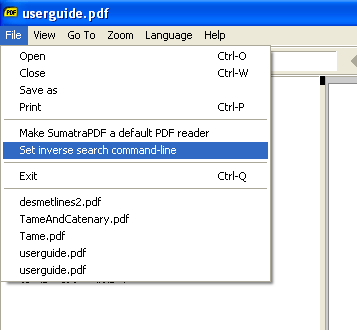
\includegraphics[height=9cm]{sumatrapdf1.PNG}}
\centerline{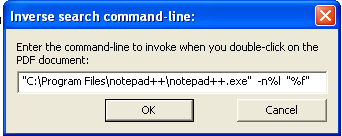
\includegraphics[height=5cm]{sumatrapdf2.PNG}}
\centerline{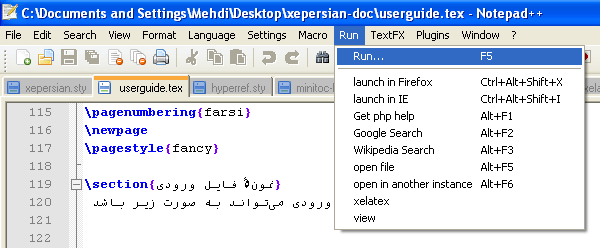
\includegraphics[height=5cm]{notepad7.PNG}}
\centerline{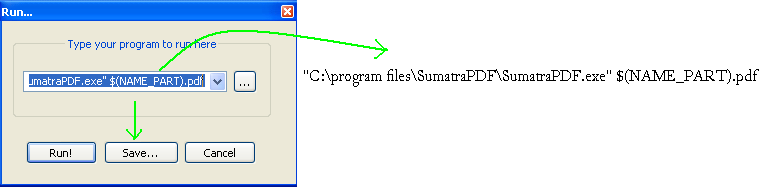
\includegraphics[height=5cm]{notepad8.PNG}}
\centerline{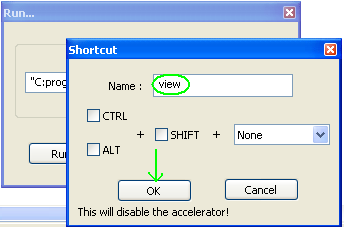
\includegraphics[height=5cm]{notepad9.PNG}}

بعد از انجام این کارها، بعد از اولین بار پردازش فایل، از منوی \lr{Run} گزینهٔ \lr{view} را انتخاب کنید تا فایل پی.دی.اف باز شود. حال بعد از هر بار پردازش،
فایل پی.دی.اف به طور خودکار آپدیت می‌شود. برای استفاده از خاصیت \lr{Inverse Search} یا جستجوی معکوس باید بستهٔ \lr{pdfsync} را در فایل ورودی خود
فراخوانی کنید. در این صورت با دو بار کلیک کردن بر یک نقطه از فایل پی.دی.اف به خط متناظر در \lr{notepad++} می‌روید. توجه داشته باشید که نسخه‌ای 
از \lr{SumatraPDF} را نصب کرده باشید که قابلیت جستجوی معکوس را داشته باشد. این نسخه را می‌توانید از آدرس زیر دریافت کنید

\begin{roman}
\verb+http://parsilatex.org/pdfreader/SumatraPDF.rar+
\end{roman}

و آن را در پوشهٔ زیر قرار دهید

\begin{roman}
\verb+C:\Program Files\SumatraPDF+
\end{roman}

\end{document}
